\documentclass[12pt,letterpaper]{article}
\usepackage[utf8]{inputenc}
\usepackage{amsmath}
\usepackage{amsfonts}
\usepackage{amssymb}
\usepackage{cancel}
\usepackage[hmargin=2cm,vmargin=2cm]{geometry}
\usepackage{graphicx}
\usepackage{subfig}
\usepackage{setspace}
\DeclareGraphicsExtensions{.pdf,.eps,.png,.jpg}

\newcommand{\proofend}{\mbox{ }\hfill$\Box$\\}
\newcommand{\pdf}[2]{\frac{\partial #1}{\partial #2}}
\newcommand{\pdt}[1]{\frac{\partial #1}{\partial t}}
\newcommand{\ddf}[2]{\frac{\mathrm{d} #1}{\mathrm{d} #2}}
\newcommand{\ddt}[1]{\frac{\mathrm{d} #1}{\mathrm{d} t}}
\newcommand{\ee}[1]{\cdot10^{#1}}
\newcommand{\eqqref}[1]{Equation \ref{#1}}
\newcommand{\dv}{\Delta v}
\newcommand{\dy}{\Delta y}
\newcommand{\dd}{\Delta }

\begin{document}

{
\centering
\part*{Untimed Dispersion Compensation for Ultrafast Electron Pulses}

\subsection*{Peter Hansen, Cory Baumgarten, Herman Batelaan, Martin Centurion\\
University of Nebraska-Lincoln\\
Department of Physics and Astronomy, Lincoln NE 68588\\
Email: mcenturion2@unlnotes.unl.edu}
}

\begin{abstract}
We propose an electron dispersion compensator (EDC) to compress ultrafast electron pulses for use at a target. 
The idea, borrowed from the optical dispersion compensator, is to use a pair of magnetic fields to deflect the electron beam, separating the electron trajectories by energy in space.
A different delay can be applied to each of energies based on their position with a Wien filter allowing for untimed compensation.
The EDC with a size of tens of centimeters is shown to compress an electron pulse back down to sub-femtosecond durations for use with Ultrafast Electron Diffraction and Ultrafast Electron Microscopy. 

PACS nrs.: 41.85.Ct, 41.85.-p, 42.65.Re
\end{abstract}

   \section{Introduction}

Ultrafast Electron Microscopy (UEM) and Ultrafast Electron Diffraction (UED) are techniques that are used to study the dynamics of molecular motion. 
To do this, short electron pulses are used to ``stroboscopically'' illuminate the molecules. 
Electron pulse durations are limited to about 100 fs, while molecular dynamics extends into the low femto-second regime. 
Additionally, electronic motion can currently only be investigated directly with recollision approaches. 
A technique to deliver very short electron pulses on a target may extend UEM and UED into a regime that allows all molecular motion to be studied, and may allow the study of electronic motion of arbitrary targets.

Pulsed electron sources with pulse durations below 100 fs \cite{Bat} and even at sub-cycle duration (2.7 fs at 800 nm) have been reported \cite{hommelhoff}.  
For these electron sources, the pulse has an appreciable energy spread of typically about 1 eV independent of energy. 
At typical energies for UEM and UED, the arrival time spread at a target is limited to about 100 fs. 
It is clear that a technique is required that reduces the temporal spread. 
Proposals for temporal lenses call for pulsed laser beams \cite{PNAS} or pulsed RF cavities \cite{Kraus} to affect the velocity of the electrons so that they regroup at the target. 
In this paper, we discuss an alternative idea to overcome the problem.

We borrow an idea from optics, an optical dispersion compensator, and propose to use magnetic fields and a Wien filter to construct an  electron dispersion compensator. 
The differences between our electron dispersion compensator and the above mentioned solutions \cite{PNAS,Kraus} is that the electron dispersion compensator is time independent, so like the optical dispersion compensator, it does not have to be synchronized with the electron pulses. 
A drawback is that this system can at best produce a pulse width as short as the one we start with. 
However, current electron source produce pulse widths well into the regime beneficial for UED and UEM. \cite{Kraus}

\begin{figure}[tb]
   \centering
   \subfloat[Electron Dispersion Compensator]{\label{setup_e}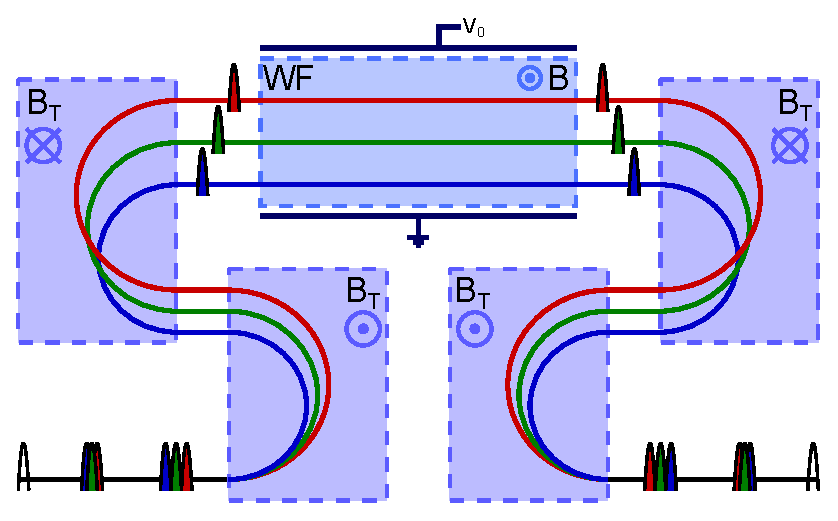
\includegraphics[width=.45\textwidth]{Setup}}
   \hspace{4mm}
   \subfloat[Optical Dispersion Compensator]{\label{setup_o}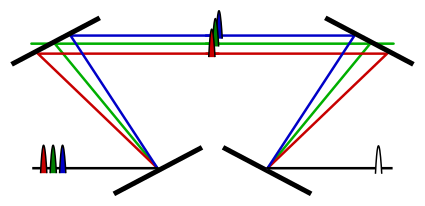
\includegraphics[width=.45\textwidth]{optical}}
   \caption{
   (a) Proposed setup for the Electron Dispersion Compensator (EDC), comprised of two sets of two turning magnetic fields and a Wien filter. 
   The different colors represent different energy electrons with the higher energies in red and the lower energies in blue. 
   Green represents the average energy electron. 
   (b) Optical Dispersion Compensator (ODC) which heavily influenced the design of the EDC. 
   The colors correspond to the different wavelengths in the light pulse where red is the longest and blue is the shortest.
   }
\end{figure}

The electron dispersion compensator (EDC), in Figure \ref{setup_e}, is modelled after the optical dispersion compensator (ODC), in Figure \ref{setup_o}.  
The first element in the optical dispersion compensator is an angled grating which disperses the light to different angles according to wavelength.  
In the EDC, the first magnetic field points perpendicular to the plane of motion and turns the electrons with a radius proportional to their velocity. 
A second angled grating in the ODC redirects the light to a path parallel to the incoming path but separated spatially by wavelength. 
Similarly, a second magnetic field turns the electrons back around, resulting in the same parallel paths, spatially separated by velocity. 
A mirror image of the two angle gratings will recombine the beam back to its original form; likewise, two magnetic fields will recombine the electron pulse. 
Since light in a vacuum has a linear dispersion relation, the phase velocity $v_{p\gamma}$ is equal to the group velocity $v_{g\gamma}$, that is $v_{p\gamma}=v_{g\gamma}=c$ where $c$ is the speed of light. 
An electron pulse has a quadratic dispersion relation, that is $v_{pe} = 2 v_{ge} = \frac{p_e^2}{2m_e}$ where $p_e$ is the electron momentum, and $m_e$ is the electron mass.

The compensation $\Delta t$ in the ODC is accomplished through the path length difference $\Delta l$, by $\Delta t=\Delta l/c$. 
For the EDC, $\Delta t$ depends on a velocity change $\Delta v$, so $\Delta t = l\dv /v_0^2$ where $l$ is the path length. 
We use a Wien Filter (WF), that is, a pair of crossed magnetic and electric fields to introduce the change in velocity.
The fields are tuned in such a way that the electrons with average velocity $v_0$ experience no net force, that is $E=v_0 B$ where $E$ is the magnitude of the electric field and $B$ is the 
Higher energy electrons (red paths in Figure \ref{setup_e}) enter the WF at a higher potential and are slowed down, while the lower energy electrons (blue paths in Figure \ref{setup_e}) enter at a lower potential and speed up. 
After the electrons exit the filter, they return to their initial velocity.
The higher energy electrons leave the filter later than the lower energy electrons.
The higher energy electrons will catch up to the slower ones, recreating the short pulse that was generated at the source. 

Notice the symmetry in Figure \ref{setup_e}. 
The whole system, including relative electron position is symmetric about the center of the Wien Filter. 
If the filter causes the electrons to have the same horizontal position at its center, then the desired compensation will be achieved. 

\section{Theory}
\subsection{Assumptions}
To begin the analysis we make the following assumptions:
\begin{enumerate}
   \item The velocity spread $\dv$ in the electron pulse is small with respect to the average velocity $v_0$. \label{smallspread}
   \item Deflection $\dy$ in the Wien filter is small with respect to the radius of curvature $r$ in the deflection magnets. (check later)
      \label{deflect}
   \item The delay caused by the fringe fields around the Wien Filter is negligible with respect to the delay inside the filter.
      \label{fringe}
   \item The pulse is a single electron pulse with uncertainty limited duration. Note that classical evolution of a Gaussian distribution in free space evolves in the same was as predicted by Quantum Mechanics.
   \item The electron source is point-like.
      \label{pointlike}
\end{enumerate}
Assumption \ref{smallspread} is reasonable since electron beams typically have a energy spread $\dd K.E.$ of 0.3 eV. 
For an energy of 3 keV, which will be used throughout this paper, $\dd K.E./K.E. \approx 10^{-4}$.
We will treat how Assumption \ref{deflect} affects the pulse later as well as calculating the fringe fields to verify Assumption \ref{fringe} is a good approximation. 

For this derivation, the motion is contained in the x-y plane with the electron pulse initially in the x-direction. 

\subsection{Deflection in the first two B-fields}
The deflection from the first two magnetic fields is  $4r$ where $r$ is the path radius of the electron in the magnetic field $B_T$:
\begin{equation}
4r=\frac{4mv}{eB_T}
\label{radius}
\end{equation}
where $m$ is the mass of the electron, $e$ is the elementary charge, $v$ is the velocity and $B_T$ is the magnitude of the turning B-fields. 
The separation $\dy$ between the paths after these two fields is
\begin{equation}
   \dy = \frac{4m\dv}{eB_T}
   \label{dy}
\end{equation}
where $\dv$ is the difference between the electron's velocity $v$ and the average velocity $v_0$. 

\subsection{Inside the Wien Filter}
Next, each electron enters the Wien filter at a position $\dy$. 
The electric field is created by two plates a distance $h$ apart and at voltages $\pm V$.
The group velocity $v_g$ of two different electron pulses entering the potential at different locations separated by $\dy$ and thus a difference of potentials $\dd V$ is given from equations 5-6 in Hasselbach \cite{hasselbach}.
\begin{align*}
   \dd V &= 2V \frac{\dy}{h} \\
   v_g = v_0 \pm \dv_g &= v_0 \pm \dd V \sqrt{\frac{e}{8 m U_a}}
\end{align*}
where $\dv_g$ is the change in group velocity and $U_a$ is the potential used to accelerate the electrons to their average kinetic energy, $\frac{1}{2}mv_0^2$.
Now we can write the change in velocity using the electric field $E=V/h$ and $U_a=mv_0^2/2e$
\begin{align}
   \dv_g&=\dd V \sqrt{\frac{e}{8 m U_a}} \nonumber \\
   \dv_g&= 2V \frac{\dy}{h} \sqrt{\frac{e}{8 m U_a}} \nonumber \\
   \dv_g&= 2 E \dy \sqrt{\frac{e^2}{4 m^2 v_0^2 }} \nonumber \\
   \dv_g&=\frac{Ee\dy}{mv_0} 
   \label{dvg}
\end{align}

We can combine \eqqref{dy} and \ref{dvg} to find the velocity change of an electron with an initial velocity $v_0+\dv$.
\begin{equation}
   \dv_g=\frac{4E}{v_0B_T}\dv
   \label{dvg2}
\end{equation}

\subsection{Calculate the delay}

The total time through the filter is $T_{WF}=d/v_g$ where $d$ is the length of the filter. 
The relative delay $\dd T_{WF}$ is 
\begin{equation}
\dd T_{WF}=\frac{d}{v_0^2}\dv_g=\frac{4 E d}{B_T v_0^3}\dv
\label{twf}
\end{equation}

Finally, we can compare the relative delay in the filter to the pulse duration that is due to the initial velocity spread. 
We start with the how the pulse width $\sigma_x$ changes with time \cite{tannoudji} and use the substitution $\sigma_{x}=\sigma_T v_0$ to find the pulse duration $\sigma_T$ as a function of time.
\begin{align}
   \sigma_x^2(t) &= \sigma_{x0}^2 +\left(\frac{\hbar t}{2 m \sigma_{x0}}\right)^2 \nonumber \\
   \frac{\sigma_x^2(t)}{v_0^2} &= \frac{\sigma_{x0}^2}{v_0^2} +\left(\frac{\hbar t}{2 m v_0 \sigma_{x0}}\right)^2 \nonumber \\
   \sigma_T^2(t) &= \sigma_{T0}^2 +\left(\frac{\hbar t}{2 m v_0^2 \sigma_{T0}}\right)^2
   \label{sigt1}
\end{align}
For $\sigma_T\gg\sigma_{T0}$, \eqqref{sigt1} becomes
\begin{equation}
   \sigma_T(t) = \frac{\hbar t }{2mv_0^2\sigma_{T0}}
   \label{sigt2}
\end{equation}
To make sure that the above classical treatment is valid, we estimate the initial pulse duration. 
It is limited by the uncertainty relation $\Delta U \sigma_T= \hbar/2$ where $\Delta U$ is the energy spread, so
\begin{equation}
   \sigma_{T0} = \frac{\hbar}{2\dd U}= \frac{\hbar}{2mv_0\dv}
   \label{t0}
\end{equation}
and substituting \eqqref{t0} into \ref{sigt2} gives
\begin{equation}
   \sigma_T(t) = \frac{\hbar t }{2mv_0^2\left(\frac{\hbar}{2mv_0\dv}\right)} =\frac{ \dv}{v_0} t
   \label{sigt}
\end{equation}

For compensation to be effective, the relative delay from \eqqref{twf} must be opposite the pulse duration would be at the target.
\begin{align}
   \dd T_{WF} &= -\sigma_T(t) \nonumber\\
   \frac{4 E d}{B_T v_0^3}\dv &= -\frac{ \dv}{v_0} t \nonumber \\
   \frac{4 E d}{B_Tv_0} &= - v_0 t
   \label{vtrel}
\end{align}
We ignore the time spent in the magnetic fields since the different velocities travel in different trajectories which result in a constant transit time through the magnetic fields. 
Since the transit time is the same for all trajectories is the same, the propagation through the magnetic fields does not contribute to the time delay. 
Letting the total propagation distance be $l=v_0 t$ we can get constraints for the system. 
\begin{align}
   \frac{4 E}{B_Tv_0} &= -\frac{l}{d}
   \label{result}
\end{align}
Experimentally, we are free to choose the average velocity $v_0$ and the ratio $l/d$ which is the distance to the target over the Wien filter length. 
This constrains the ratio $E/B_T$ based on those choices.

%We calculate the  velocity change $\dv_{WF}$ due to the change in potential that is set up by the electric field $E$ by looking at energy conservation.
%\begin{align} 
%T_i &=  U+T_f \\
%\frac{1}{2}m\left( v_0 +\dv\right)^2 &= - Ee\Delta y + \frac{1}{2} m v_{WF}^2\\
%\frac{1}{2}m\left( v_0 +\frac{eB_T}{4m}\dy \right)^2 &= - Ee\dy + \frac{1}{2} m v_{WF}^2 \\ 
%\left( v_0 +\frac{eB_T}{4m}\dy \right)^2 &= - \frac{2Ee}{m} \dy+ v_{WF}^2
%\end{align}
%\[
%v_{WF} =\sqrt{\left( v_0 +\frac{eB_T}{4m}\dy \right)^2+\frac{2Ee}{m} \dy} 
%\]
%\[
%v_{WF} =v_0 + \dy\frac{(2v_0\frac{eB_T}{4m}+\frac{2Ee}{m})}{2v_0}
%\]
\section{Simulation}

To verify this analytical result, we used a simulation written in Fortran to solve the differential equations of motion with a Runge-Kutta-Verner fifth-order method. 
We used the equations of motion given by Newton's equations and the Lorentz force.
\[
\frac{\partial^2\vec{r}}{\partial t^2} = \frac{e}{m}\left( \pdt{\vec{r}} \times \vec B + \vec E\right)
\]
For each run, the starting position is set to the origin. 
The initial velocity is set to a specific angle and magnitude. 
We chose angles of 1 mrad, an energy range of $\Delta K.E./ K.E=10^{-4}$ and an energy of 3 keV which corresponds to a $v_0$ of $3.23\ee{7}$ m/s.
The electron is propagated until it reaches a boundary, for example, between an area with and without magnetic fields. When an electron is close to a boundary, that is, when the distance to the boundary $\delta\le\tau v_0$ where $\tau$ is the average time step, the step size is reduced to $\tau\ee{-5}$ up until the boundary is reached. 
Then the field values are changed and the time step is changed back to $\tau$. 

The first region is a magnetic field. 
We used a field strength of 3.1 mT which results in a radius of curvature of 5.92 cm, which can be calculated using the equation $r=mv_0/eB_T$ (\eqqref{radius}). 
For a target at a distance of 10 cm, the whole path is contained in a 25cm box. 
After the electron crosses the first boundary again, the direction of the magnetic field is reversed.
When the next boundary is crossed, the fields are turned off, simulating a period of free space before entering the Wien filter. 
When the electron crosses the boundary of the beginning and the end of the Wien filter, the velocity is affected and calculated using energy conservation. 
The velocity in the x-direction after the boundary $v_{xf}$ is calculated using 
\[
v_{xf}=\sqrt{v_{xi}^2+\frac{2 E e}{m}\dy}
\]
where $v_{xi}$ is the velocity in the x-direction before the boundary, $\dy$ is the distance from the center of the pulse, $y_0$, and the $\pm$ sign indicates the electron entering or leaving the filter.
We first run a test trajectory with the velocity $v_0$ and no initial angle which represents the center of the pulse. 
We store the position of this electron as it enters the filter as $y_0$ and use the arrival time at the final target position $x=l$ for our stopping criteria.
The field values are set in the filter to the values of the crossed electric and magnetic fields determined by the theory (\eqqref{result}. 
The magnetic field in the Wien filter can be tuned to reduce the deflection caused by the uniform electric field. This deflection will be considered below. 
  
In one dimension, three points is sufficient to determine up to quadratic spreading of electrons as a function of velocity or angle spread. To simulate both velocity and angle spread, we set nine different initial conditions with varying initial angles and initial velocities. 
The these are propagated through the series of fields until the end time determined from the test trajectory is reached.
To calculate the width of the pulse at the target, we find the difference between the maximum and minimum x-positions of the end of each trajectory.

To test the accuracy of the simulation, we decreased the time steps used and verified that the resulting pulse width did not change. 
We have also compared the path given by the simulation to an analytical approximation of the trajectories.
In Figure \ref{fmi}, the simulation is plotted against these equations. This shows that the trajectories produced by the simulation are reasonable compared to the analysis. 
A third test we used was to propagate an electron back through the fields after reaching the end and measuring how far from the starting point they were after the same amount of time. Figure \ref{tnb} shows the results from this test. In the x-direction we have a error spread for one propagation around 0.01 $\mu$m 


\begin{figure}[tb]
   \centering
   \subfloat[Filter motion]{\label{fmi}\includegraphics[width=.45\textwidth]{FilterMotionInset.PNG}}
   \hspace{4mm}
   \subfloat[Retrace propagation test]{\label{tnb}\includegraphics[width=.45\textwidth]{thereandback.PNG}}
   \caption{
   (a) The simulated trajectory compared to the analytical trajectory. The inset shows the difference between the analytical and simulated results
   (b) Results of propagating the electrons back through the system. The error of the two propagations is given by the distance each point is from the origin. 
   }
\end{figure}

\begin{figure}[tb]
   \centering
   \subfloat[Pulse Spread (9 paths)]{\label{endpoint2}\includegraphics[width=.45\textwidth]{endpoint2.PNG}}
   \hspace{4mm}
   \subfloat[Pulse Spread ($\sim$900 paths]{\label{endpoint1}\includegraphics[width=.45\textwidth]{endpoint1.PNG}}
   \caption{
   (a) Here, the ends of all nine trajectories are show. The pulse center is located at the origin.
   (b) Same as (a), but with a uniform distribution between the upper and lower limit in both angle and energy spread. 
   }
\end{figure}
\section{Results}
For an initial pulse with an angle spread $\Delta \theta$ of 1 mrad and energy spread $\Delta K.E/K.E.$ of 3.25$\ee{-4}$, the resulting pulse width is 3.825$\ee{-3} \mu$m which corresponds to a pulse duration of 118 as. This is well into the useful range for UED and UEM. Figure \ref{endpoint2} and \ref{endpoint1}

In order to achieve such a small pulse width, a non-uniform magnetic field must be used in the Wien filter. 
If the Wien filter magnetic field strength $B_{WF}$ is set to $E/v_0$ then the Lorentz Force is balanced only for the electrons that have velocity $v_0$ and enter at the center of the filter. 
All other electrons will have a slight deflection exiting the filter, which is amplified by the remaining two magnetic fields. 
The assumption that the turning magnetic fields do not contribute any time delay only holds for electrons that enter perpendicular to the boundary. 
If they enter at an angle, the path length differs by $4\theta r$, so even a minimal deflection of 0.01 mrad would translate to a time delay of 61 fs (2 orders of magnitude larger than our target pulse width). 
This can be correct by tuning $B_{WF}$ to match the velocity based on the vertical position of the electron. That is 
\begin{equation}
   B_{WF}(y)=\frac{E}{v_{WF}(y)}
\end{equation}
where $v_{WF}$ is the velocity an electron should have after entering the filter. If the electron has no initial angle, it enters the filter according to \eqqref{dy} and experiences a velocity change according to \eqqref{dvg} resulting in 
\begin{align}
   v_{WF}&=v_0+\dv+\dv_g \nonumber \\
   v_{WF}&=v_0+\frac{eB_T}{4m} \dy+\frac{Ee}{mv_0}\dy \nonumber \\
\end{align}
Using \eqqref{result}, we find 

\begin{align}
   B_{WF}&=\frac{E}{v_0+\frac{eB_T}{4m} \dy+\frac{eE}{mv_0}\dy} \\
   B_{WF}&=\frac{E}{v_0+\left(1 -\frac{l}{d}\right)\frac{eB_T }{4 m}\dy} \label{bwf1}\\
   B_{WF}&=\frac{E}{v_0}\left(1-\left(1 -\frac{l}{d}\right)\frac{eB_T }{4 m v_0}\dy\right) \label{bwf2}
\end{align}
using a first order Taylor expansion around $\dy=0$.
Changing the $B_{WF}$ to depend on $\dy$ results in theoretically perfect compensation for electrons without an initial angle, but introduces complications to the analytical solution for electrons with an initial angle. 

When an electron enters the Wien filter at an angle, it oscillates back and forth in the y-direction, perpendicular to the propagation.
This along with the y-dependence of the magnetic field set up a differential equation of motion that has no analytic solution. 
By making a few approximations, the we were apply to analytically reproduce these complex electron paths within 10\% error. 
We approximated the acceleration in the x-direction as zero and assume that the velocity in the x-direction is determined by the potential, that is
\begin{equation}
   v_{xWF} = \sqrt{(v+\dv)^2 \cos^2 \theta - \frac{2eE}{m} \dy} \approx (v+\dv) \cos \theta -\frac{eE}{v_0 m} \dy
   \label{vxwf}
\end{equation}
Using \eqqref{bwf2} and \ref{vxwf}, we can write the equations of motion in the y-direction as
\begin{equation}
   \dot{v}_y=\frac{e}{m}\left( -v_{xWF}(y) B_{WF}(y) +E \right)
   \label{motion}
\end{equation}
These equations of motion, shown in Figure \ref{fmi}, are still off by about 10\% after propagating through the filter.

\section{Acknowledgments}
I would like to acknowledge the Undergraduate Creative Activities and Research Experiences (UCARE) at University of Nebraska-Lincoln and the National Science Foundation (NSF) for founding this research.

I would like to thank Martin Centurion for starting this idea off. 

Also, Herman Batelaan has been an invaluable advisor and teacher who has spent many hours working out issues and keeping me motivated. 



\pagebreak
\begin{thebibliography}{9}
   \bibitem{hommelhoff} 
      Hommelhoff P, Kealhofer C and Kasevich M A 2006 Phys. Rev. Lett. 97 247402 
   \bibitem{Bat}
      B Barwick et al 2007 New J. Phys. 9 142 doi:10.1088/1367-2630/9/5/142
   \bibitem{PNAS}
      Baum P and Zewail A H 2006 Proc. Natl Acad. Sci. USA 103 16105
   \bibitem{Kraus}
      L Veisz et al 2007 New J. Phys. 9 451 doi:10.1088/1367-2630/9/12/451
   \bibitem{hasselbach}
      Nicklaus M and Hasselbach F 1993 Wien filter: a wave-packet-shifting device for restoring longitudinal coherence in charged-matter-wave interferometers Phys. Rev. A 48 152
   \bibitem{tannoudji}
      Cohen-Tannoudji C, Diu B and Laloe F. Quantum Mechanics. 2006 (Wiley-Interscience, New York) 
\end{thebibliography}

\end{document}

